\documentclass[12pt, twoside]{article}
\usepackage[letterpaper, margin=1in, headsep=0.5in]{geometry}
\usepackage[english]{babel}
\usepackage[utf8]{inputenc}
\usepackage{amsmath}
\usepackage{amsfonts}
\usepackage{amssymb}
\usepackage{tikz}
%\usetikzlibrary{quotes, angles}

\usepackage{graphicx}
\usepackage{enumitem}
\usepackage{multicol}

\usepackage{fancyhdr}
\pagestyle{fancy}
\fancyhf{}
\renewcommand{\headrulewidth}{0pt} % disable the underline of the header

\fancyhead[RE]{\thepage}
\fancyhead[RO]{\thepage \\ Name: \hspace{3cm}}
\fancyhead[L]{BECA / Dr. Huson / 10th Grade Geometry\\* 14 March 2019}

\begin{document}
\subsubsection*{8-8 Homework: Similar triangles, dilation ratios}
 \begin{enumerate}

  \begin{multicols}{2}
  [\item A translation maps triangle $ABC$ onto triangle $XYZ$.] \vspace{0.5cm}
    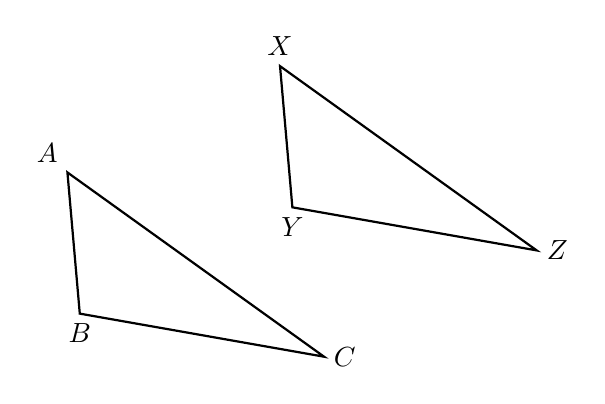
\begin{tikzpicture}[scale=0.9]
      \coordinate [label=above left:$A$](A) at (95:2);
      \coordinate [label=below:$B$](B) at (0, 0);
      \coordinate [label=right:$C$](C) at (-10:3.5);
      \draw [thick] (A)--(B)--(C)--cycle;

      \draw [thick, xshift=3cm, yshift=1.5cm] (95:2) node[above]{$X$}--
      (0,0) node[below]{$Y$}--
      (-10:3.5) node[right]{$Z$}--cycle;
    \end{tikzpicture}\\
    Circle the true statement(s). The $\triangle$s are ...
    \begin{enumerate}
      \item congruent, but not similar
      \item similar, but not congruent
      \item both congruent and similar
      \item neither congruent nor similar
    \end{enumerate}
  \end{multicols}  \vspace{1cm}

  \item Given $\triangle JKL \sim \triangle MNO$. $m\angle K = 31^\circ$ and $m\angle M = 53^\circ$.\\
  Find the measure of $\angle L$. \vspace{3cm}

 \item Triangle $ABC$ is dilated with a scale factor of $k$ centered at $A$, yielding $\triangle ADE$, as shown. Given $AB=12$, $BC=15$, $AC=18$, and $DE=20$. \\[0.25cm] Find $AD$, $CE$, and $k$ (the scale factor). \vspace{0.5cm}
 \begin{center}
     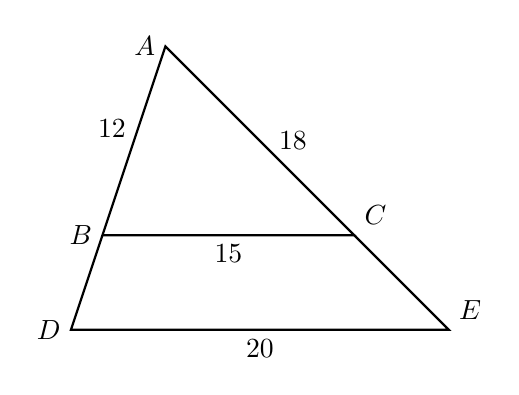
\begin{tikzpicture}[scale=0.4]
       \draw [thick]
       (0,0)node[left]{$B$}--
       (8,0)node[above right]{$C$}--
       (2,6)node[left]{$A$}--cycle;
       \draw [thick]
       (0,0)--
       (-1,-3)node[left]{$D$}--
       (11,-3)node[above right]{$E$}--(8,0);
       \node at (4,0)[below]{$15$};
       \node at (5.3, 3)[right]{$18$};
       \node at (0.3, 2.8)[above]{$12$};
       \node at (5,-3)[below]{$20$};
     \end{tikzpicture}
   \end{center}

\newpage


\item Given $\triangle ABP$ and $\triangle JKP$ as shown below. $\overline{AB} \parallel \overline{JK}$ with $AB=5$, $PA=4$, $PB=2$, and $PK=5$.\\[0.25cm]
Find $PJ$ and $JK$.\\[0.5cm]
  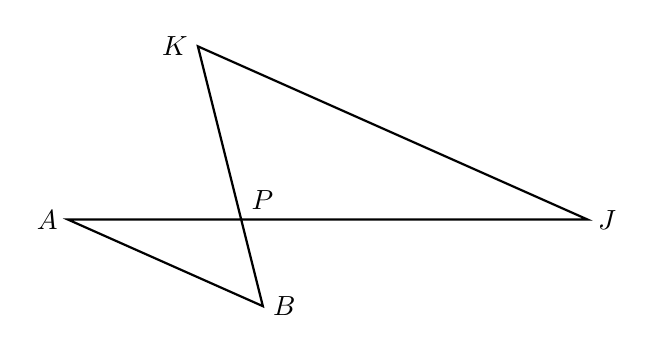
\begin{tikzpicture}[scale=1.1]
      \draw [thick]
        (0.25,-1)node[right]{$B$}--
        (-0.5,2)node[left]{$K$}--
        (4,0)node[right]{$J$}--
        (0,0)node[above right]{$P$}--
        (-2,0)node[left]{$A$}--cycle;
    \end{tikzpicture}
    \vspace{3cm}


    \item Triangle $ADE$ and its midline $\overline{BC}$ are drawn, with $B$ the midpoint of $\overline{AD}$ and $C$ the midpoint of $\overline{AE}$. The two medians $\overline{AE}$ and $\overline{AE}$ are drawn, as shown, intersecting in point $F$, the centroid.\\[0.25cm]
    $\triangle FCB \sim \triangle FDE$ with scale factor $k=2$.\\[0.25cm]
    Given $BC=9$, find $DE$. \\[0.25cm] Given $BF=5$, find $FE$. %\vspace{1cm}
    \begin{center}
        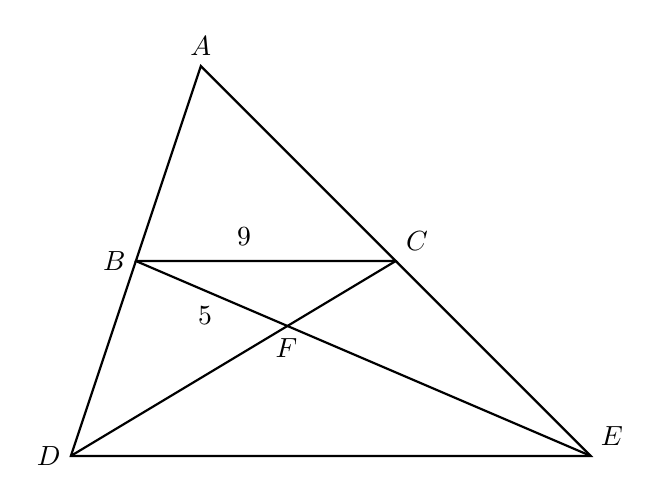
\begin{tikzpicture}[scale=0.55]
          \draw [thick]
          (0.5,1.5)node[left]{$B$}--
          (6.5,1.5)node[above right]{$C$}--
          (2,6)node[above]{$A$}--cycle;
          \draw [thick]
          (0.5,1.5)--
          (-1,-3)node[left]{$D$}--
          (11,-3)node[above right]{$E$}--(6.5,1.5);
          \draw [thick] (0.5,1.5)--(11,-3);
          \draw [thick] (6.5,1.5)--(-1,-3);
          \node at (3,2.5)[below]{$9$};
          \node at (3.5, -0.5)[right]{$F$};
          \node at (2.1, -0.2)[above]{$5$};
          %\node at (-0.7, -1)[above]{$5$};
        \end{tikzpicture}
      \end{center} \vspace{1cm}

\end{enumerate}

\newpage

\subsubsection*{8-3 Homework: Similar triangles, dilation ratios}
 \begin{enumerate}

 \item Given $\triangle ABP$ and $\triangle JKP$ as shown below. $\overline{AB} \parallel \overline{JK}$. $AP=5.7$, $JP=11.4$, and $JK=14.8$. Find $AB$.
 \begin{center}
   \begin{tikzpicture}[scale=1.4]
       \draw [thick]
         (0.25,-1)node[right]{$B$}--
         (-0.5,2)node[left]{$K$}--
         (4,0)node[right]{$J$}--
         (0,0)node[above right]{$P$}--
         (-2,0)node[left]{$A$}--cycle;
     \end{tikzpicture}
     \end{center}

     \vspace{2cm}

 \item Triangle $ABC$ is dilated with a factor of $\frac{3}{2}$ centered at $A$, yielding $\triangle ADE$, as shown. Given $AB=10$, $BC=12$, and $AC=14$. \\[0.25cm] Find $AD$, $AE$, and $DE$. \vspace{1cm}
 \begin{center}
     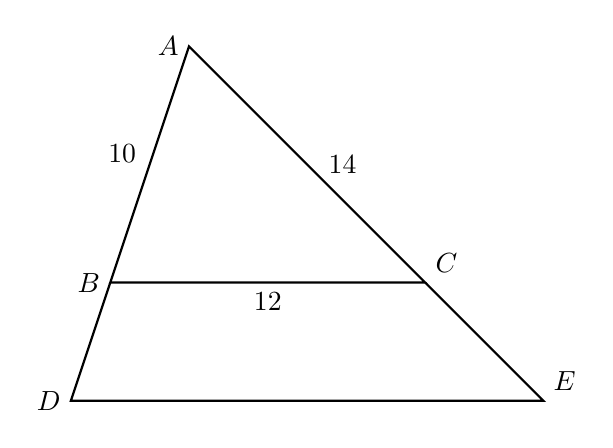
\begin{tikzpicture}[scale=0.5]
       \draw [thick]
       (0,0)node[left]{$B$}--
       (8,0)node[above right]{$C$}--
       (2,6)node[left]{$A$}--cycle;
       \draw [thick]
       (0,0)--
       (-1,-3)node[left]{$D$}--
       (11,-3)node[above right]{$E$}--(8,0);
       \node at (4,0)[below]{$12$};
       \node at (5.3, 3)[right]{$14$};
       \node at (0.3, 2.8)[above]{$10$};
     \end{tikzpicture}
   \end{center}



   \newpage

    \item The vertices of $\triangle JKL$ have the coordinates $J(-4,-2)$, $K(-1,-1)$, and $L(-2,3)$, as shown below. \\[0.5cm]
    Apply a translation of $(x,y) \rightarrow (x+7, y+2)$ to $\triangle JKL$ and then reflect the image across the $x$-axis. Draw both images $\triangle J'K'L'$ and $\triangle J''K''L''$ on the set of axes below, labeling the vertices.
    \begin{center}
      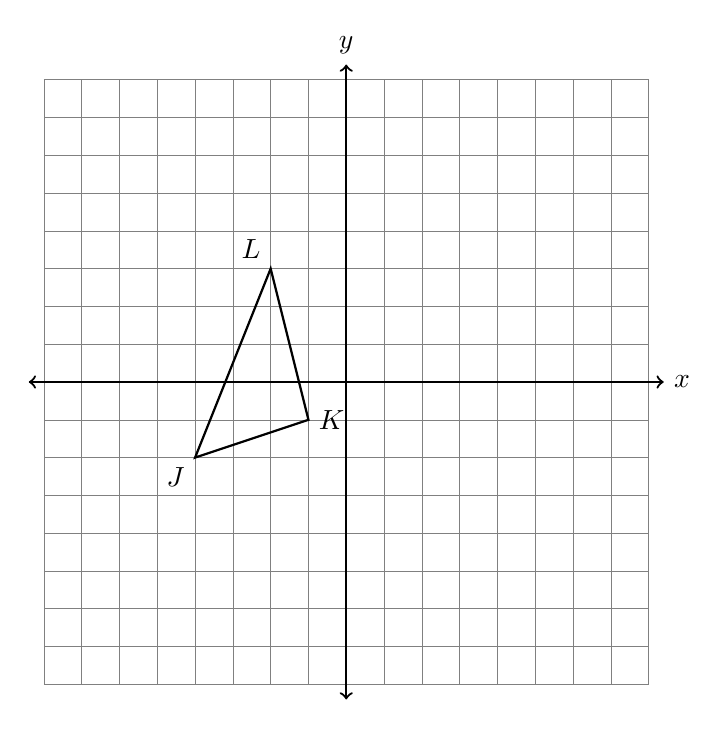
\begin{tikzpicture}[scale=.48]
        \draw [help lines] (-8,-8) grid (8,8);
        \draw [thick, <->] (-8.4,0) -- (8.4,0) node [right] {$x$};
        \draw [thick, <->] (0,-8.4)--(0,8.4) node [above] {$y$};

        \draw [thick]
        (-4,-2) node[below left] {$J$}--
        (-1,-1) node[right] {$K$}--
        (-2,3) node[above left] {$L$}--
        cycle;
      \end{tikzpicture}
    \end{center}

 \item A rotation of $90^\circ$ is applied to $\triangle ABC$, mapping it onto $\triangle PQR$, as shown.  \\[0.25cm]
 Which triangle has the larger area, or are they equal? Justify your answer.\\
     \begin{tikzpicture}[scale=.48]
       \draw [thick, <->] (-7.4,0) -- (10.4,0) node [right] {$x$};
       \draw [thick, <->] (0,-5.4)--(0,10.4) node [above] {$y$};

       \draw [thick]
       (4,-2) node[below left] {$A$}--
       (8,2) node[right] {$B$}--
       (1,1) node[above right] {$C$}--cycle;

       \draw [thick]
       (2,4) node[right] {$P$}--
       (-2,8) node[above] {$Q$}--
       (-1,1) node[below left] {$R$}--cycle;

     \end{tikzpicture}


\newpage

  \item Using a compass and straightedge, construct the perpendicular bisector of $\overline{BB'}$  \\[0.25cm]
  What transformation has been applied to map $\triangle ABC$ on to $\triangle A'B'C'$? \vspace{2cm}
      \begin{center}
      \begin{tikzpicture}%[scale=.48]
        %\draw [thick, <->] (-7.4,0) -- (10.4,0) node [right] {$x$};
        %\draw [thick, <->] (0,-6.4)--(0,10.4) node [above] {$y$};

        \draw [thick]
        (5,-1) node[below left] {$A$}--
        (8,2) node[right] {$B$}--
        (1,0) node[below left] {$C$}--cycle;

        \draw [thick]
        (-1,5) node[right] {$A'$}--
        (2,8) node[above] {$B'$}--
        (0,1) node[below left] {$C'$}--cycle;

      \end{tikzpicture}
    \end{center}

\end{enumerate}
\end{document}
